\documentclass[10pt]{amsart}

\usepackage{graphicx}
\usepackage[margin=0.5in]{geometry}

\begin{document}
\begin{figure}
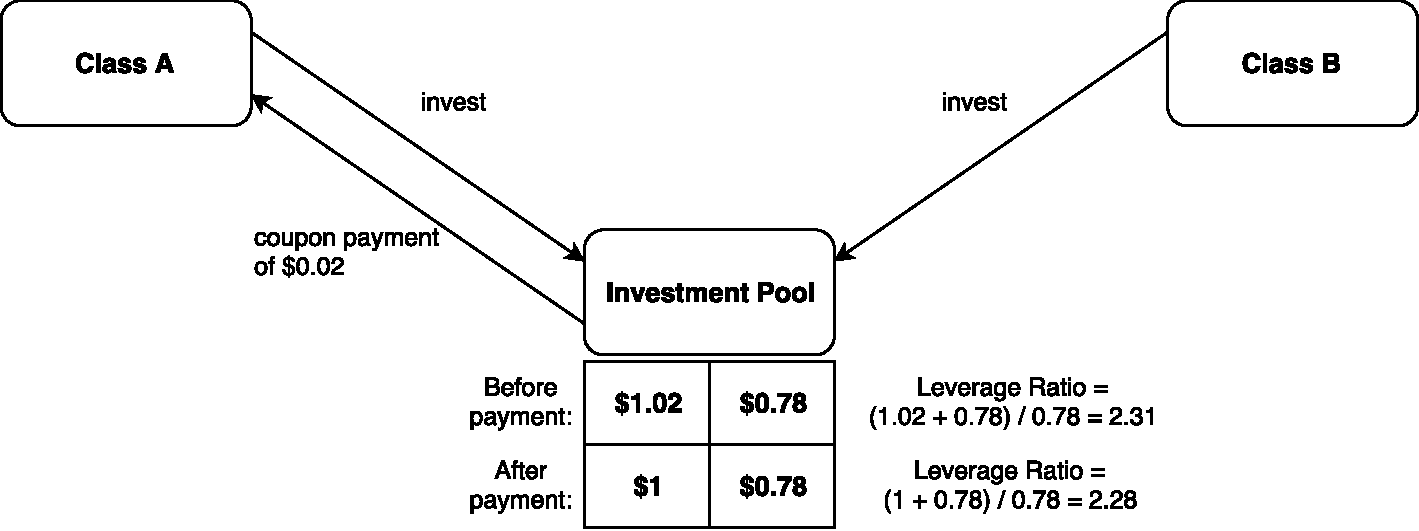
\includegraphics[width=\textwidth]{periodic.pdf}
\caption{Periodic Reset. At beginning, Class A and B each invest \$1 in Eth. On periodic reset dates (per 100 days), Class A receives coupon payment \$0.02, i.e. at daily rate 0.02\%.}
\end{figure}

\begin{figure}
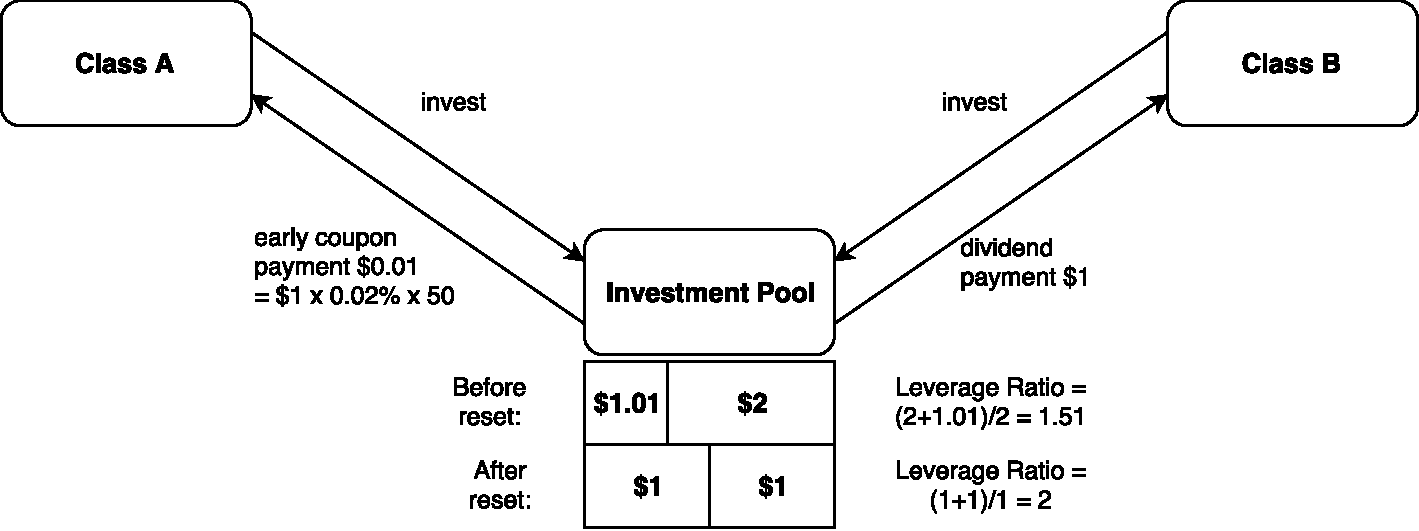
\includegraphics[width=\textwidth]{upward.pdf}
\caption{Upward Reset. After half a year, Class B NAV grows to \$2, therefore an upward reset occurs. Class A NAV equals \$1.01, where \$0.01 is half-year accrued coupon. On this date, Class A receives \$0.01 coupon payment, and Class B receives \$1 dividend payment.}
\end{figure}

\begin{figure}
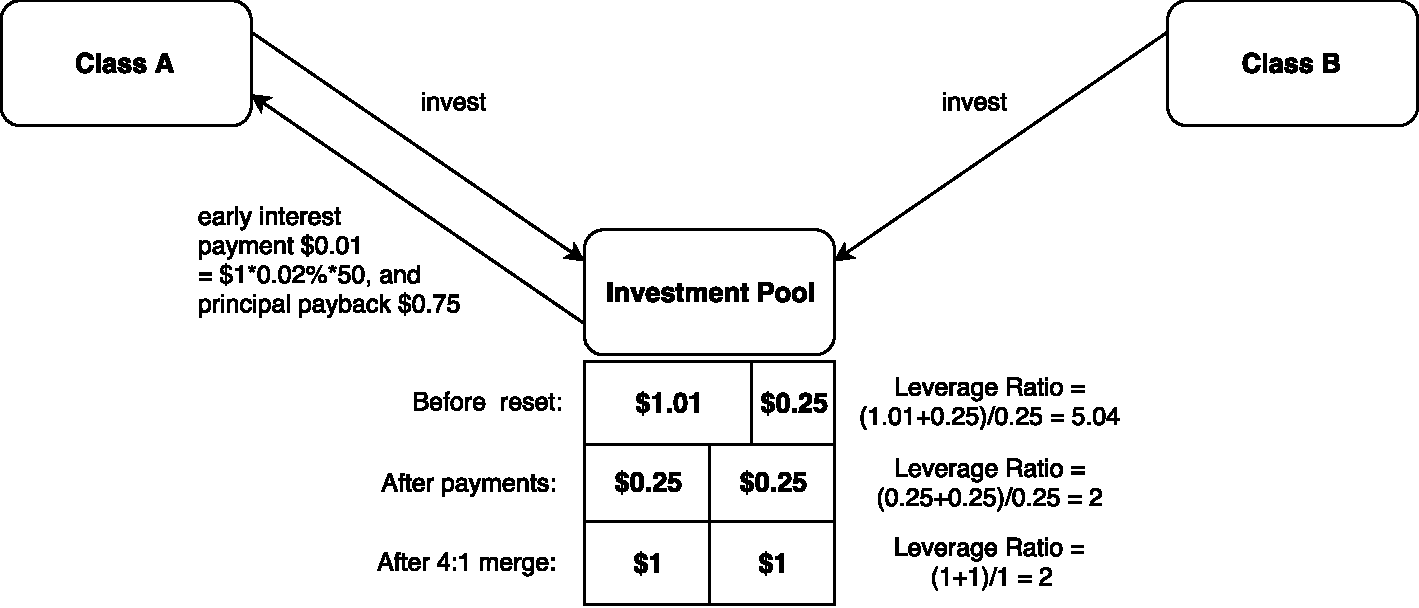
\includegraphics[width=\textwidth]{downward.pdf}
\caption{Downward Reset. After another half a year, Class B NAV drops to \$0.25, therefore an downward reset occurs. Again, Class A NAV equals \$1.01, where \$0.01 is half-year accrued coupon. On this date, Class A receives \$0.01 coupon payment, as well as \$0.75 principal payback. Then, Class A and B undergo a 4:1 merge, so that both have NAV equal to \$1.}
\end{figure}

\begin{figure}
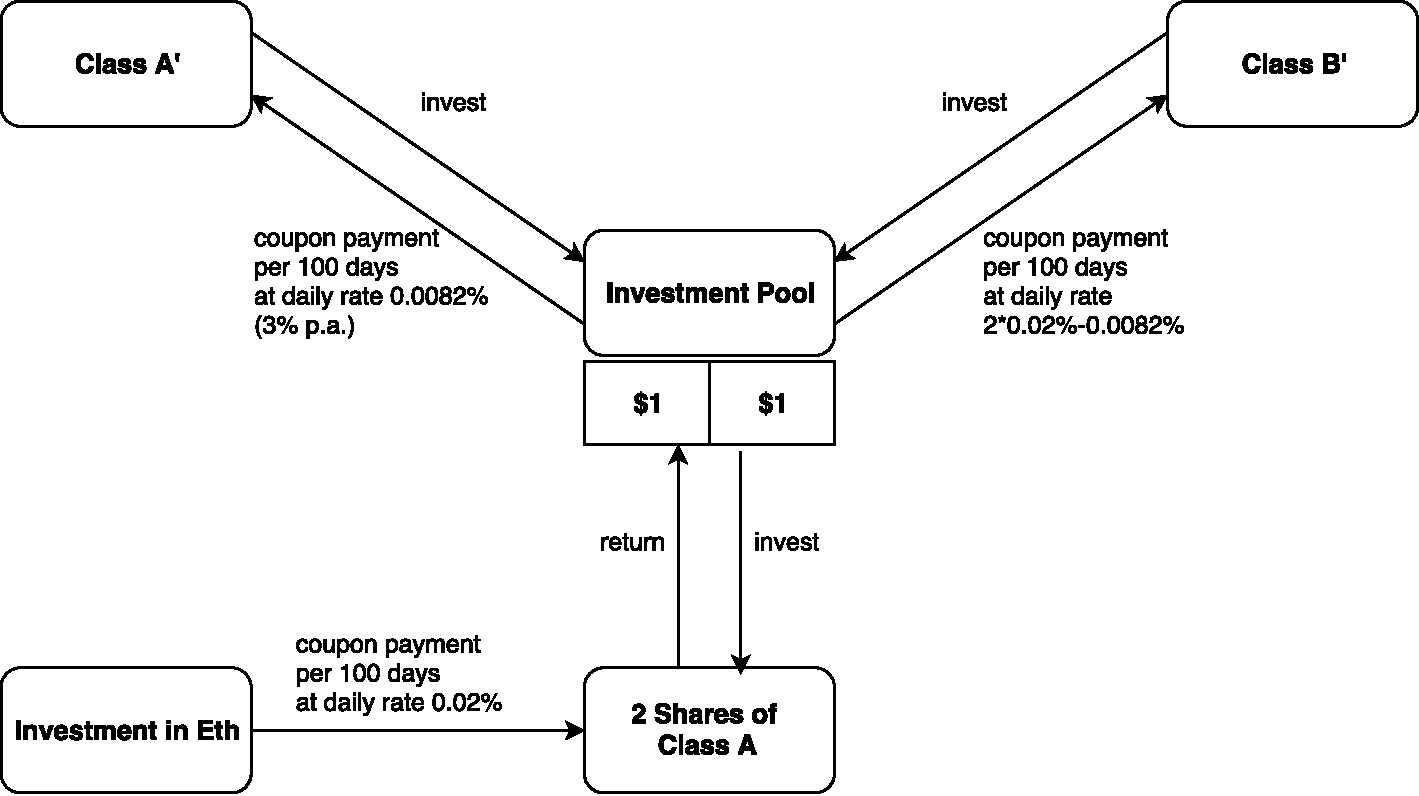
\includegraphics[width=\textwidth]{Ap_periodic.pdf}
\caption{Periodic Reset of Class A$^\prime$. This figure corresponds to Figure 1. At beginning, Class A$^\prime$ and B$^\prime$ each invest \$1, in a total of 2 shares Class A. On periodic reset dates (per 100 days), 2 shares of Class A receives coupon payment \$0.04, i.e. at daily rate 0.02\%. Within this \$0.04, \$0.0082 is paid to Class A$^\prime$, and the remaining is paid to Class B$^\prime$.}
\end{figure}

\begin{figure}
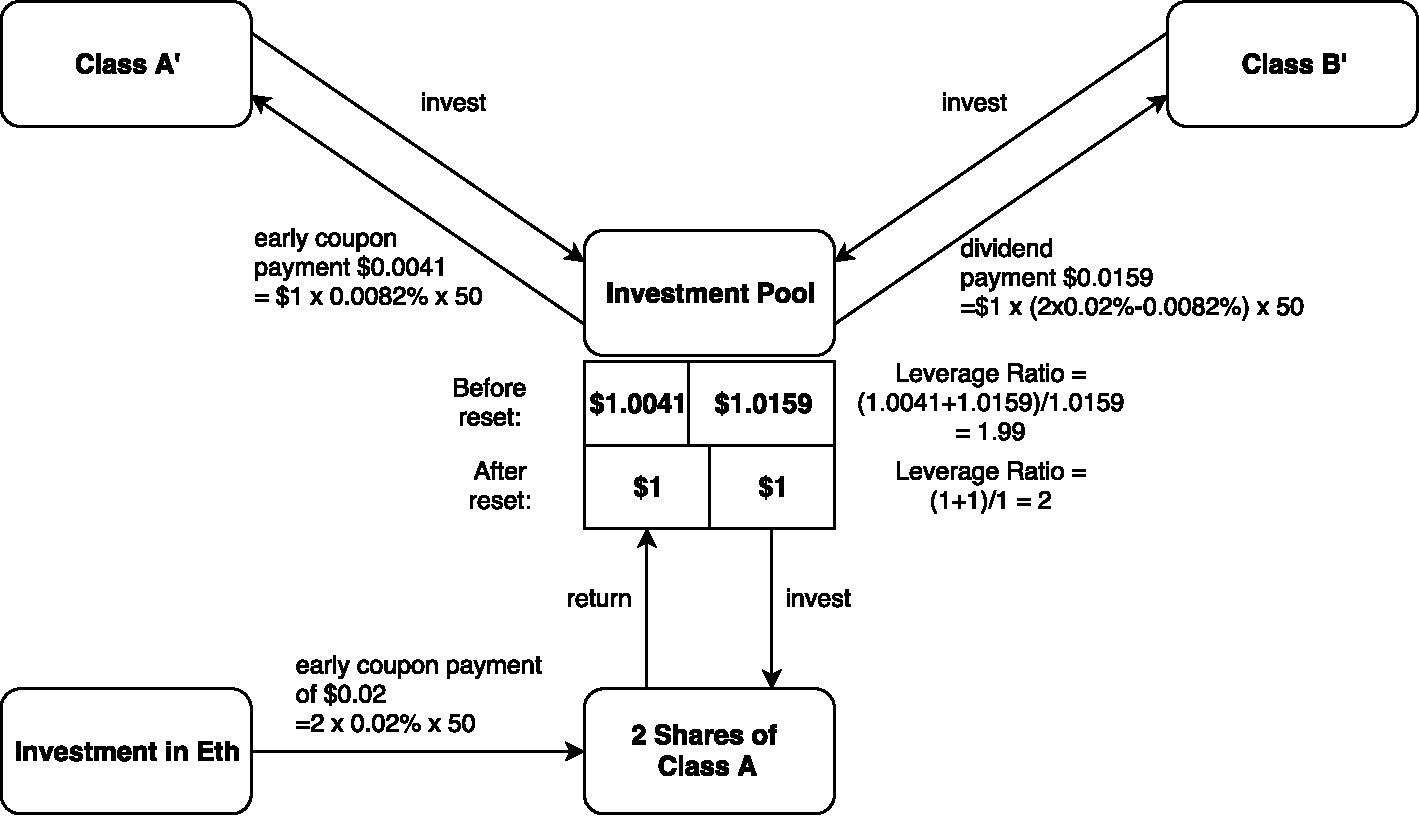
\includegraphics[width=\textwidth]{Ap_upward.pdf}
\caption{Upward Reset of Class A$^\prime$. This figure corresponds to Figure 2. After half a year, Class B NAV grows to \$2, therefore an upward reset occurs. Class A NAV equals \$1.01, where \$0.01 is half-year accrued coupon. On this date, each Class A receives \$0.01 coupon payment, so 2 shares of Class A have \$0.02 coupon. Within this \$0.02, \$0.0041 is paid to Class A$^\prime$, and the remaining is paid to Class B$^\prime$}
\end{figure}

\begin{figure}
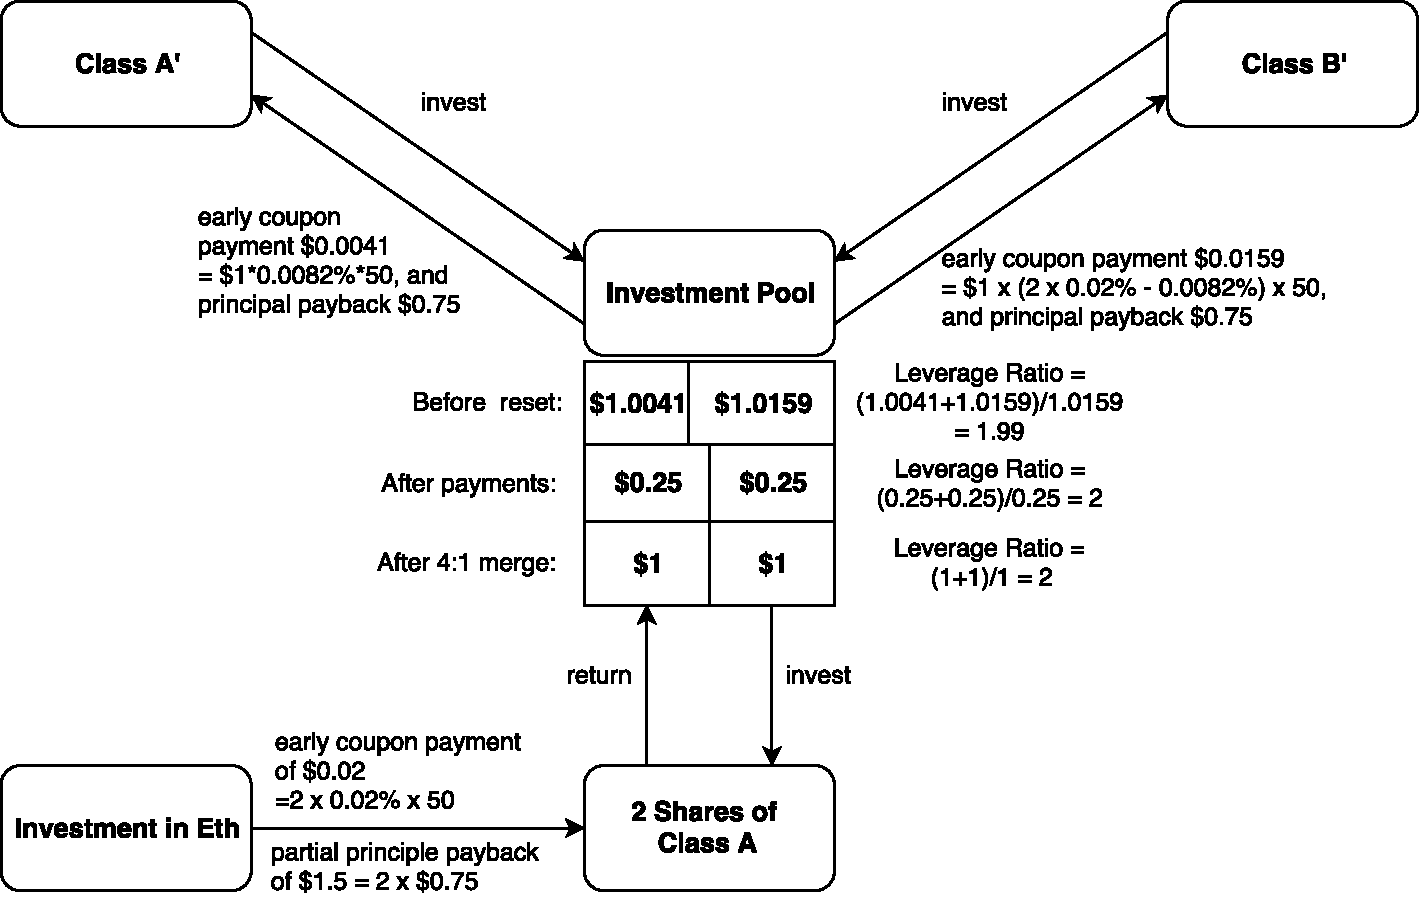
\includegraphics[width=\textwidth]{Ap_downward.pdf}
\caption{Downward Reset of Class A$^\prime$. This figure corresponds to Figure 3. After another half a year, Class B NAV drops to \$0.25, therefore an downward reset occurs. Again, Class A NAV equals \$1.01, where \$0.01 is half-year accrued coupon. On this date, Class A receives \$0.01 coupon payment, as well as \$0.75 principal payback. Then, Class A undergoes a 4:1 merge. Therefore, 2 shares of Class A receives \$2*(0.01+0.75). Within this amount, \$0.0041+0.75 goes to Class A$^\prime$, and the remaining goes to Class B$^\prime$. Then, both Class A$^\prime$ and B$^\prime$ undergo a 4:1 merge, so that their NAV return to \$1.}
\end{figure}

\begin{figure}
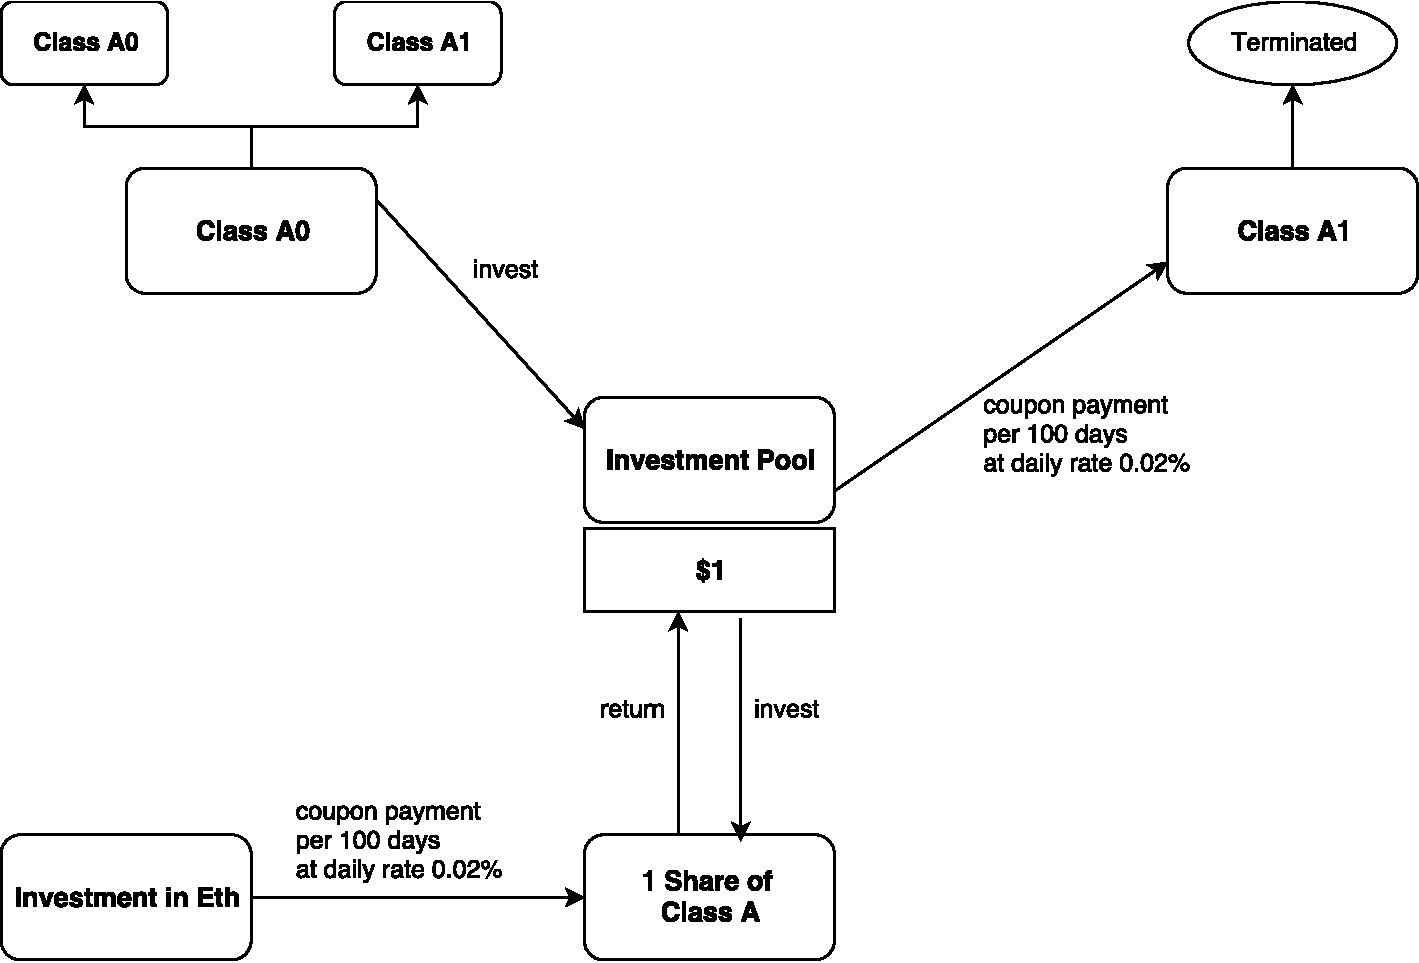
\includegraphics[width=\textwidth]{A0_periodic.pdf}
\caption{Periodic Reset of Class A0. This figure corresponds to Figure 1. At beginning, Class A0 \$1 in 1 share of Class A, but receives no coupon. Class A1 does not invest, but receives coupon payment \$0.02 on periodic reset dates (per 100 days), i.e. at daily rate 0.02\%. That is, Class A1 receives all the coupon payment of Class A. After the coupon payment, Class A1 is terminated, and 1 Class A0 is split into 1 new Class A0 and Class A1.}
\end{figure}

\begin{figure}
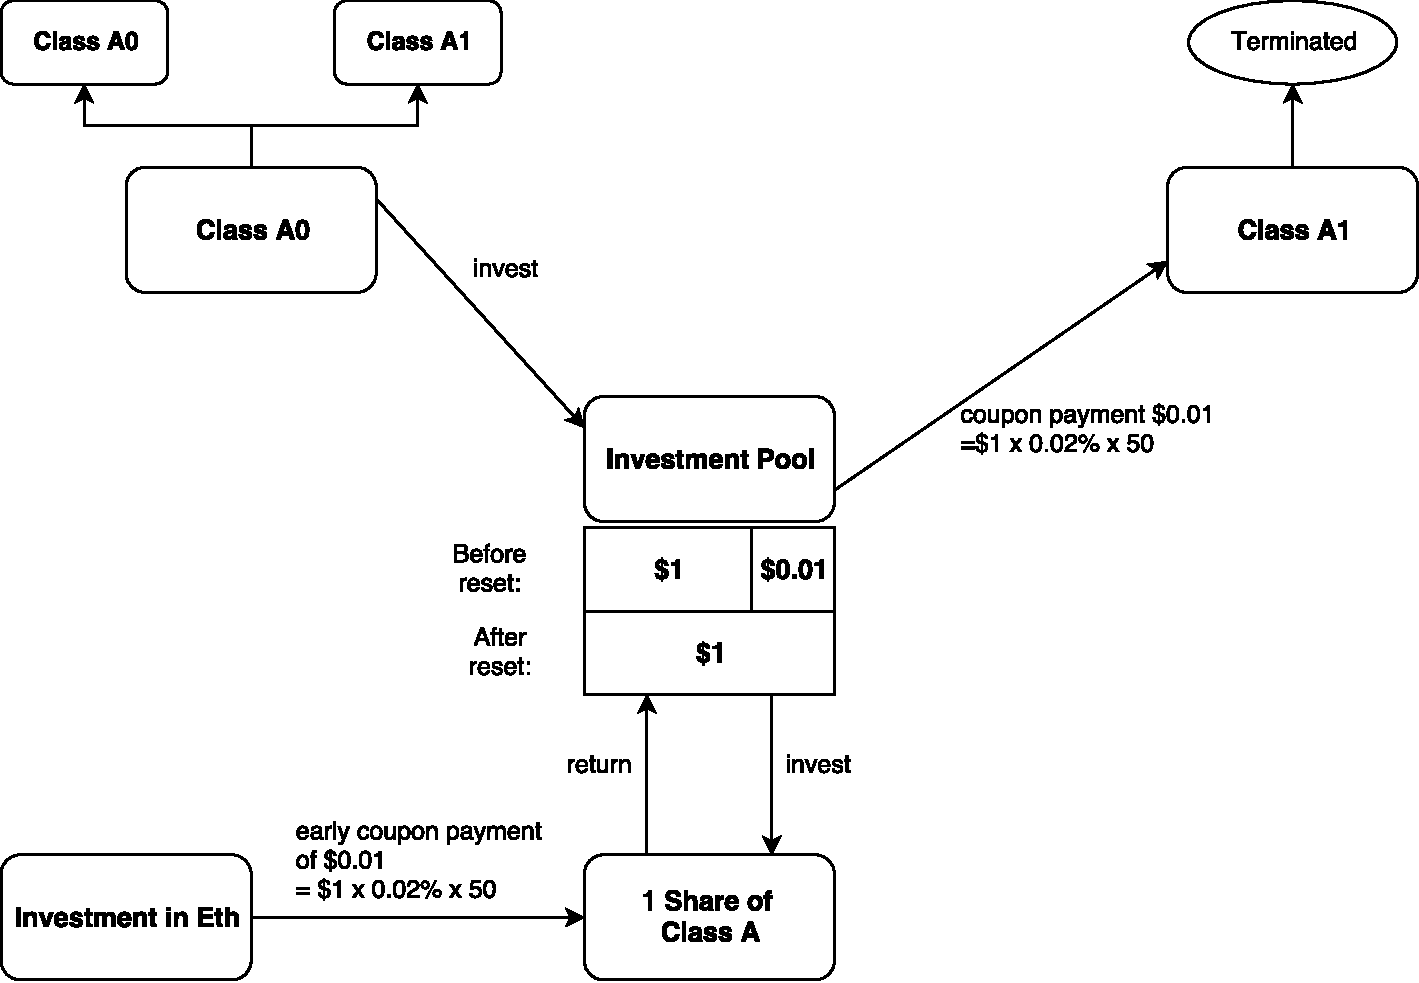
\includegraphics[width=\textwidth]{A0_upward.pdf}
\caption{Upward Reset of Class A0. This figure corresponds to Figure 2. After half a year, Class B NAV grows to \$2, therefore an upward reset occurs. Class A NAV equals \$1.01, where \$0.01 is half-year accrued coupon. On this date, each Class A receives \$0.01 coupon payment. This \$0.01 is paid out to Class A1. After the coupon payment, Class A1 is terminated, and 1 Class A0 is split into 1 new Class A0 and Class A1.}
\end{figure}

\begin{figure}
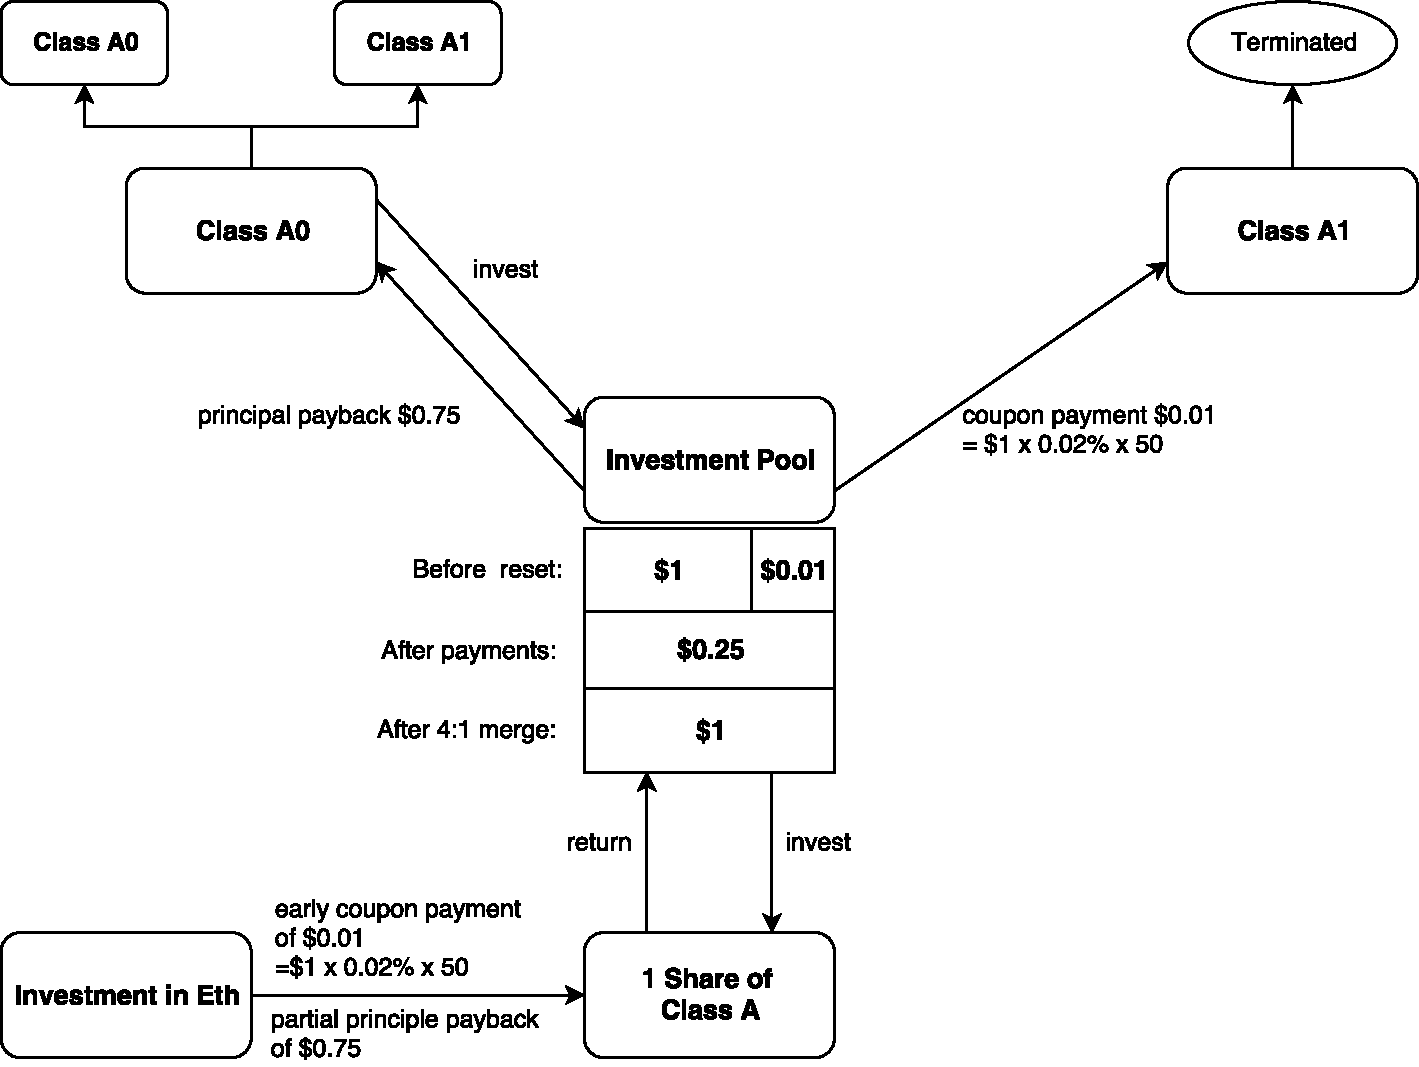
\includegraphics[width=\textwidth]{A0_downward.pdf}
\caption{Downward Reset of Class A0. This figure corresponds to Figure 3. After another half a year, Class B NAV drops to \$0.25, therefore an downward reset occurs. Again, Class A NAV equals \$1.01, where \$0.01 is half-year accrued coupon. On this date, Class A receives \$0.01 coupon payment, as well as \$0.75 principal payback. Then, Class A undergoes a 4:1 merge. Within this amount, \$0.01 goes to Class A1, and \$0.75 goes to Class A0. After the coupon payment, Class A1 is terminated, Class A0 undergoes a 4:1 merge, and then 1 Class A0 is split into 1 new Class A0 and Class A1.}
\end{figure}


\end{document}